\documentclass[a4paper,dvipdfmx]{jsarticle}%jsarticleがよい

  % amsmath, amssymb
  % AMS(American Mathematical Society, 米国数学会)のパッケージ
  % 数学記号やらギリシャ文字やら。この2つは一緒に宣言しておく。
  \usepackage{amsmath,amssymb,nccmath}

  % 画像の挿入、テキストや図の拡大縮小・回転
  \usepackage[hiresbb]{graphicx}%hiresbb=high resolution bounding box 高解像度

  %下線とかを引けるように
  \usepackage{ulem}

  %hereパッケージの置き換え
  \usepackage{float}

  % 関連した図を並べて挿入するため
  \usepackage{subcaption}

  % itemのlabel変更を簡単に
  \usepackage{enumitem}

  % URLを書くために使う
  \usepackage{url}

  % 定理等を枠で囲む
  \usepackage{ascmac}

  \usepackage{textcomp}
  %普通のμとかを使う
  \usepackage{textgreek}
  %ギリシャ文字を普通に使う

  %コメント複数行できるように
  \usepackage{comment}

  %化学式を変換してくれる http://doratex.hatenablog.jp/entry/20131203/1386068127
  \usepackage[version=3]{mhchem}

  \usepackage{array}

  %ベクトルの太字表記
  \usepackage{bm}

  \usepackage{xcolor}

  %subsubsectionまで目次に入れる
  \setcounter{tocdepth}{3}

  %余白とかをなんか良い感じにしてくれる呪文
  \setlength{\textwidth}{\fullwidth}
  \setlength{\textheight}{40\baselineskip}
  \addtolength{\textheight}{\topskip}
  \setlength{\voffset}{-0.2in}
  \setlength{\topmargin}{0pt}
  \setlength{\headheight}{0pt}
  \setlength{\headsep}{0pt}
%以上プリアンブル

%----------------------------------------------------------------------------

%タイトル
\title{2D拡散方程式}
 \author{武者野 拓也}
 \date{20120/1/15}

\begin{document}
  \maketitle
  2D NS方程式:
  \begin{align}
    &\dfrac{\partial u}{\partial t} + \dfrac{\partial uu}{\partial x} + \dfrac{\partial vu}{\partial y} = -
    \dfrac{1}{\rho}\dfrac{\partial p}{\partial x} + \nu \left(\dfrac{\partial^2 u}{\partial x^2} + \dfrac{\partial^2 u}{\partial y^2}\right)\\
    &\dfrac{\partial u}{\partial t} + \dfrac{\partial uv}{\partial x} + \dfrac{\partial vv}{\partial y} = -\dfrac{1}{\rho}\dfrac{\partial p}{\partial y} + \nu \left(\dfrac{\partial^2 v}{\partial x^2} + \dfrac{\partial^2 v}{\partial y^2}\right)
  \end{align}
  を無次元化し、非圧縮の条件\(\nabla \cdot \bm{v} = 0\)を課すと次のようになる。
  \begin{align}
    &\dfrac{\partial u}{\partial x} + \dfrac{\partial v}{\partial y} = 0\\
    &\dfrac{\partial u}{\partial t} + u\dfrac{\partial u}{\partial x} + v\dfrac{\partial u}{\partial y} = - \dfrac{\partial p}{\partial x} + \dfrac{1}{Re}\left( \dfrac{\partial^2 u}{\partial x^2} + \dfrac{\partial^2 u}{\partial y^2} \right)\\
    &\dfrac{\partial v}{\partial t} + u\dfrac{\partial v}{\partial x} + v\dfrac{\partial v}{\partial y} = - \dfrac{\partial p}{\partial y} + \dfrac{1}{Re}\left( \dfrac{\partial^2 v}{\partial x^2} + \dfrac{\partial^2 v}{\partial y^2} \right)
  \end{align}
  これを最も簡単にした、次の拡散方程式を計算領域\( 0 \leq x \leq L_x, 0 \leq y \leq L_y \) で数値的に解くことにする。
  \begin{equation}
    \dfrac{\partial f}{\partial t} = \kappa \left( \dfrac{\partial^2 f}{\partial x^2} + \dfrac{\partial^2 f}{\partial y^2} \right)
  \end{equation}
  x方向の格子点が\(N_x\)個、y方向の格子点が\(N_y\)個となるように格子間隔を\( \Delta x = L_x/(N_x-1), \Delta y = L_y/(N_y-1) \)とした。また、時間ステップ幅\(\Delta t\) は、次のように設定した。
  \begin{equation}
    \Delta t = 0.2 \min(\Delta x, \Delta y)^2 /\kappa
  \end{equation}
  これらを用いて、時間微分項には前進差分、区間微分項には中心差分を適用し、拡散方程式を次のように差分化する。
  \begin{equation}
    \dfrac{f_{i,j}^{n+1} - f_{i,j}^n}{\Delta t} = \kappa \left( \dfrac{f_{i+1,j}^n - 2f_{i,j}^n + f_{i-1,j}^n}{\Delta x^2} + \dfrac{f_{i,j+1}^n - 2f_{i,j}^n + f_{i,j-1}^n}{\Delta y^2} \right)
  \end{equation}
  したがって、時間更新式は次のようになる。
  \begin{equation}
    f_{i,j}^{n+1} = f_{i,j}^n + \Delta t \kappa \left( \dfrac{f_{i+1,j}^n - 2f_{i,j}^n + f_{i-1,j}^n}{\Delta x^2} + \dfrac{f_{i,j+1}^n - 2f_{i,j}^n + f_{i,j-1}^n}{\Delta y^2} \right)
  \end{equation}
  これを様々な初期条件、\(\kappa\)や\(\mu\)の値において次のような初期条件のもと計算した。
  \begin{figure}[H]%fig単品ver
    \centering
    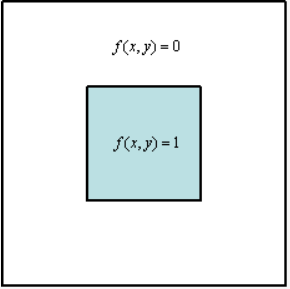
\includegraphics[width=0.4\columnwidth]{boundary.png}
    \caption{境界条件}
    \label{boundary}
  \end{figure}%

  \begin{equation}
    \dfrac{\partial f}{\partial t} + u\dfrac{\partial f}{\partial x} + v\dfrac{\partial f}{\partial y} = 0
  \end{equation}
\end{document}
